\documentclass[10pt]{article}

\usepackage[letterpaper]{geometry}
\usepackage{enumerate,verbatim,mdwlist,multirow}
\usepackage{fancyhdr}
\usepackage{linguex}
\usepackage[colorlinks=true,linkcolor=blue]{hyperref}
\usepackage{multicol}

%Packages needed for trees
\usepackage{amsfonts,amsmath,amssymb}
\usepackage[varg]{txfonts}
\usepackage{qtree}

%%%%%%%%%%%%%%%%%%%%%%%%%%%%%%%%%%%%%%%%%%%%%
%% Represent categorical logic graphically %%
%%%%%%%%%%%%%%%%%%%%%%%%%%%%%%%%%%%%%%%%%%%%%

\usepackage{tikz}
\usepackage{xstring}

\usetikzlibrary{shapes,backgrounds}
\tikzstyle{every node}=[font=\tiny] 

%%%%%%%%%%%%%%%%%%%%%%%%%%%%%%%%
%% Draw squares of Opposition %%
%%%%%%%%%%%%%%%%%%%%%%%%%%%%%%%%

\def\oppsquare{(-1.5,1) node[above left]{$All$} -- (1.5,1) node[above right]{$No$} -- (1.5,-1) node[below right]{$Some-not$} -- (-1.5,-1) node[below left]{$Some$} -- (-1.5,1)}
\def\oppcross{(-1.5,1) -- (1.5,-1) node[sloped,above,pos=0.3]{contra} node[sloped,above,pos=0.7]{dictory} (-1.5,-1) -- (1.5,1) node[sloped,above,pos=0.3]{contra} node[sloped,above,pos=0.7]{dictory}}

\def\sqroppMod{%
  \begin{scope}
    \draw \oppsquare;
    \draw \oppcross;
    \draw (-1.75,0) node[rotate=90] {undet.};
    \draw (0,1.25) node {undet.};
    \draw (0,-1.25) node {undet.};
    \draw (1.75,0) node[rotate=90] {undet.};
  \end{scope}
}

\def\sqroppTrad{%
  \begin{scope}
    \draw \oppsquare;
    \draw \oppcross;
    \draw (-1.75,0) node[rotate=90] {subalt.};
    \draw (0,1.25) node {contrary};
    \draw (0,-1.25) node {subcontrary};
    \draw (1.75,0) node[rotate=90] {subalt.};
  \end{scope}
}

%%%%%%%%%%% Turn categorical props into Venn diagrams %%%%%%%%%%%%%%%
%% \catvenn{title:<y/n>}{quantifier:<All/No/Some>}{quality:<not/>} %%
%%         {complement:<non-/>}{subject class}                     %%
%%         {complement:<non-/>}{predicate class}                   %%
%%%%%%%%%%%%%%%%%%%%%%%%%%%%%%%%%%%%%%%%%%%%%%%%%%%%%%%%%%%%%%%%%%%%%

%%%%%%%%%%%%%
%% Circles %%
%%%%%%%%%%%%%

%% Venn circles
\def\firstcircle{(0,0) circle (1cm)} 
\def\secondcircle{(0:1.5cm) circle (1cm)}
\def\thirdcircle{(60:1.5cm) circle (1cm)}

%% Overlapping and disjoint circles
\def\firstcircleN{(0,0) circle (.75cm) node [below left=.25in] {$A$}}
\def\secondcircleN{(0:2cm) circle (.75cm) node [below right=.25in] {$B$}}
\def\firstcircleA{(0,0) circle (1.25cm) node [above right] {$A$}}
\def\secondcircleA{(.125,0) circle (.75cm) node [below left=.25in] {$B$}}

%%%%%%%%%%%%%%%%%%%%%%%%%%%
%% Venn diagram template %%
%%%%%%%%%%%%%%%%%%%%%%%%%%%

\newcommand{\vennbox}[2]{%
  \draw (-1.5,-1.5) rectangle (3,1.5);
  \draw \firstcircle node [below left=.25in] {#1};
  \draw \secondcircle node [below right=.25in] {#2};
}

\newcommand{\syllbox}[3]{%
  \draw (-1.5,-1.5) rectangle (3,2.75);
  \draw \firstcircle node [below left=.25in] {#1};
  \draw \secondcircle node [below right=.25in] {#2};
  \draw \thirdcircle node [above right=.25in] {#3};
}

%%%%%%%%%%%%%%%%%%%%
%% Universal Defs %%
%%%%%%%%%%%%%%%%%%%%

\def\fillleft{%
  \begin{scope}[even odd rule, fill opacity=0.5]
    \clip \secondcircle (-1,-1) rectangle (1,1);
    \fill[blue] \firstcircle;
  \end{scope}
}

\def\fillmiddle{%
  \begin{scope}[fill opacity=0.5]
    \clip \firstcircle;
    \fill[blue] \secondcircle;
  \end{scope}
}

\def\fillright{%
  \begin{scope}[even odd rule, fill opacity=0.5]
    \clip \firstcircle (-1,-1) rectangle (2.5,1);
    \fill[blue] \secondcircle;
  \end{scope}
}

\def\fillbox{%
  \begin{scope}
    \fill[fill opacity=0.5, blue] (-1.5,-1.5) rectangle (3,1.5);
    \fill[fill opacity=1, white] \firstcircle \secondcircle;
  \end{scope}
}

%%%%%%%%%%%%%%%%%%%%%%
%% Existential Defs %%
%%%%%%%%%%%%%%%%%%%%%%

\def\xleft{%
  \node {x};
}
\def\xleftA{%
\draw (0,0) node [draw,rounded corners] {x};
}%

\def\xmiddle{%
  \node [right=.6cm] {x};
}
\def\xmidA{%
  \draw (.75cm,0) node [draw,rounded corners] {x};
}%

\def\xright{%
  \node [right=1.5cm] {x};
}

\def\xbox{%
 \node [below right=1.1cm] {x};
}

%%%%%%%%%%%%%%%%%%%
%% Draw diagrams %%
%%%%%%%%%%%%%%%%%%%

\newcommand{\catvenn}[7]{%
  \IfEqCase{#2}{%
    {All}{%
      \IfEqCase{#4}{%
	{non-}{%
	  \IfEqCase{#6}{%
	    {non-}{\fillright}%
	    {}{\fillbox}%
	  }[\PackageError{catvenn}{Undefined option to tree: pred-non}{}]%
	}%
	{}{%
	  \IfEqCase{#6}{%
	    {non-}{\fillmiddle}%
	    {}{\fillleft}%
	  }[\PackageError{catvenn}{Undefined option to tree: pred-non}{}]%
	}%
      }[\PackageError{catvenn}{Undefined option to tree: subj-non}{}]%
    }%
    {No}{%
      \IfEqCase{#4}{%
	{non-}{%
	  \IfEqCase{#6}{%
	    {non-}{\fillbox}%
	    {}{\fillright}%
	  }[\PackageError{catvenn}{Undefined option to tree: pred-non}{}]%
	}%
	{}{%
	  \IfEqCase{#6}{%
	    {non-}{\fillleft}%
	    {}{\fillmiddle}%
	  }[\PackageError{catvenn}{Undefined option to tree: pred-non}{}]%
	}%
      }[\PackageError{catvenn}{Undefined option to tree: subj-non}{}]%
    }%
    {Some}{%
      \IfEqCase{#3}{%
	{not}{%
	  \IfEqCase{#4}{%
	    {non-}{%
	      \IfEqCase{#6}{%
		{non-}{\xright}%
		{}{\xbox}%
	      }[\PackageError{catvenn}{Undefined option to tree: pred-non}{}]%
	    }%
	    {}{%
	      \IfEqCase{#6}{%
		{non-}{\xmiddle}%
		{}{\xleft}%
	      }[\PackageError{catvenn}{Undefined option to tree: pred-non}{}]%
	    }%
	  }[\PackageError{catvenn}{Undefined option to tree: subj-non}{}]%
	}%
	{}{%
	  \IfEqCase{#4}{%
	    {non-}{%
	      \IfEqCase{#6}{%
		{non-}{\xbox}%
		{}{\xright}%
	      }[\PackageError{catvenn}{Undefined option to tree: pred-non}{}]%
	    }%
	    {}{%
	      \IfEqCase{#6}{%
		{non-}{\xleft}%
		{}{\xmiddle}%
	      }[\PackageError{catvenn}{Undefined option to tree: pred-non}{}]%
	    }%
	  }[\PackageError{catvenn}{Undefined option to tree: subj-non}{}]%
	}%
      }[\PackageError{catvenn}{Undefined option to tree: not}{}]%
    }%
  }[\PackageError{catvenn}{Undefined option to tree: quant}{}]%
  
  \IfEqCase{#1}{%
    {y}{\draw (0,1.25) node {#2 #4#5 are #3 #6#7};}%
    {n}{}%
  }[\PackageError{catvenn}{Undefined option to tree: title}{}]%
  
  \vennbox{#5}{#7}%
}%

%%%%%%%%%%%%%%%%%%%%%%%%%%%%
%% Categorical syllogisms %%
%%%%%%%%%%%%%%%%%%%%%%%%%%%%

\newcommand{\filltopleft}[1]{%
  \begin{scope}[fill opacity=0.5]
    \clip \firstcircle;
    \fill[#1] \thirdcircle;
  \end{scope}
}

\newcommand{\filltopright}[1]{%
  \begin{scope}[fill opacity=0.5]
    \clip \secondcircle;
    \fill[#1] \thirdcircle;
  \end{scope}
}

\def\filltopfirst{%
  \begin{scope}[even odd rule, fill opacity=0.5]
    \clip \firstcircle (-1.5,-1.5) rectangle (3,2.75);
    \fill[green] \thirdcircle;
  \end{scope}
}

\def\filltopsecond{%
  \begin{scope}[even odd rule, fill opacity=0.5]
    \clip \secondcircle (-1.5,-1.5) rectangle (3,2.75);
    \fill[green] \thirdcircle;
  \end{scope}
}

\def\xtopleft{%
  \draw (60:.75cm) node [text=red] {x};
}

\def\xtopright{%
  \draw (30:1.3cm) node {x};
}

\def\xtopmid{%
  \draw (30:.85cm) node [text=red] {X};
}



%% Margin Setting
\geometry{hmargin={.5in,.5in},vmargin={1in,1in}}
\setlength{\parindent}{0.0in}
%\setlength{\parskip}{2mm}
\setlength{\tabcolsep}{10pt}
\setlength{\arraycolsep}{10pt}

%% Header
\setlength{\headheight}{23pt}
\pagestyle{fancy}
\fancyhead{}
\fancyhead[L]{Phil 101, f14}
\fancyhead[C]{Homework \# 3}
\fancyhead[R]{Due: Wednesday October 15, 2014 \\ Point total: 20 points}

\begin{document}

\small

\textbf{Name:}\underline{  Answer Key  }

\paragraph{The language of categorical logic}

\begin{enumerate}
 \item What is the primary difference between the \textbf{Boolean} and \textbf{Aristotelian} perspectives on categorical logic? \textbf{(1 point)}
 
 \begin{quote}
  \textit{The Boolean perspective denies that universal propositions have existential import, whereas the Aristotelian perspective demands that they do.}
 \end{quote}

\suspend{enumerate}

\vspace{.5cm}

\paragraph{Syntactic relations}

\resume{enumerate}
  \item Write the converse of \textit{Some A are non-B}: \underline{  \textit{Some non-B are A}  } \textbf{(1 point)}
  
  \item Write the obverse of \textit{No Q are S}: \underline{  \textit{All Q are non-S}  } \textbf{(1 point)}
  
  \item Write the contraposition of \textit{Some non-M are not N}: \underline{  \textit{Some non-N are not M}  } \textbf{(1 point)}
\suspend{enumerate}

\paragraph{Semantic relations}

\resume{enumerate}
  \item Assume that \textit{All A are B} is true. 
  
  Then the truth value of \textit{No A are B} is: \hspace{1cm} True \hspace{1cm} \tikz \node [draw, ellipse] {False}; \hspace{1cm} Undetermined \hspace{1cm} \textbf{(circle one, 1 point)} \\
  
  The relation that allows us to make that claim is: \underline{  \textit{Contrary}  } \textbf{(1 point)}
  
  \item Assume that \textit{Some F are G} is false. 
  
  Then the truth value of \textit{All F are G} is: \hspace{1cm} True \hspace{1cm} \tikz \node [draw, ellipse] {False}; \hspace{1cm} Undetermined \hspace{1cm} \textbf{(circle one, 1 point)} \\
  
  The relation that allows us to make that claim is: \underline{  \textit{Subalternation}  } \textbf{(1 point)}
  
\suspend{enumerate}

\paragraph{Direct inferences}

\resume{enumerate}
  \item Assume the \textbf{Boolean perspective}, and consider the direct inference: \textit{Some W are not X}. Therefore, it is false that \textit{no W are X}.
  
  \vspace{3mm}
  
  This inference is: \hspace{1cm} Valid \hspace{1cm} \tikz \node [draw, ellipse] {Invalid}; \hspace{1cm} Conditionally valid \hspace{1cm} \textbf{(circle one, 1 point)}
  
  \vspace{3mm}
  
  Justify your answer in the space below.  You may use either method for assessing the validity of direct inferences. \textbf{(2 points)}
  
  \paragraph{Method \#1:} First, we translate the conclusion using the contradictory relation from the square of opposition. This gives us: 
  
  \textit{It is false that no W are X} $\rightarrow$ \textit{Some W are x}.
  
  Then, we construct venn diagrams for each of the propositions:
  
  \begin{center}
  \begin{tikzpicture}
   \catvenn{y}{Some}{not}{}{W}{}{X}
   \draw (0,-1.25cm) node {Premise};
   \begin{scope}[shift={(6cm,0)}]
    \catvenn{y}{Some}{}{}{W}{}{X}
    \draw (0,-1.25cm) node {Conclusion};
   \end{scope}
  \end{tikzpicture}
  \end{center}

  Based on these diagrams, it is clear that the conclusion says something that the premise does not.  Thus, the inference is \textit{invalid}.
  
  \paragraph{Method \#2:} First, we check the square of opposition to determine what relation the two propositions stand in.  Since we are in the Boolean perspective, we use the modern square. \textit{Some-not} and \textit{No} are on the right side of the square, which means the relation between them is \textit{undetermined}.  Thus, we can't say anything about the truth value of one given that of the other, and the inference is \textit{invalid}.
  
  \newpage
  
  \item Assume the \textbf{Aristotelian perspective}, and consider the direct inference: It is false that \textit{some R are S}. Therefore, it is false that \textit{All R are S}.
  
  \vspace{3mm}
  
  This inference is: \hspace{1cm} Valid \hspace{1cm} Invalid \hspace{1cm} \tikz \node [draw, ellipse] {Conditionally valid}; \hspace{1cm} \textbf{(circle one, 1 point)}
  
  \vspace{3mm}
  
  Justify your answer in the space below.  You may use either method for assessing the validity of direct inferences. \textbf{(2 points)}
  
  \paragraph{Method \#1:} First, we translate both propositions using the contradictory relation from the square of opposition. This gives us: 
  
  \textit{It is false that some R are S} $\rightarrow$ \textit{No R are S}, and 
  
  \textit{It is false that all R are S} $\rightarrow$ \textit{Some R are not S}.
  
  Then, we construct venn diagrams for each of the propositions:
  
  \begin{center}
  \begin{tikzpicture}
   \catvenn{y}{No}{}{}{R}{}{S}
   \xSonlyA
   \draw (0,-1.25cm) node {Premise};
   \begin{scope}[shift={(6cm,0)}]
    \catvenn{y}{Some}{not}{}{R}{}{S}
    \draw (0,-1.25cm) node {Conclusion};
   \end{scope}
  \end{tikzpicture}
  \end{center}

  Notice that the diagram for the premise includes an \tikz \node [draw, rounded corners] {X}; because we are working in the Aristotelian perspective. Based on these diagrams, the conclusion doesn't say anything that the premise does not already say.  Thus, the inference is valid. But because of the existential import, we say that the inference is \textit{conditionally valid}.
  
  \paragraph{Method \#2:} First, we check the square of opposition to determine what relation the two propositions stand in.  Since we are in the Aristotelian perspective, we use the traditional square. \textit{Some} and \textit{All} are on the left side of the square, which means the relation between them is \textit{subalternation}.  Thus, we know that falsity flows upward. Since our premise is on the bottom, and it is said to be false, we know that the conclusion must also be false, which is jsut what it says.  Thus, the inference is valid. But since we're in the Aristotelian perspective we qualify this and call it \textit{conditionally valid}.
  
\suspend{enumerate}

\paragraph{Syllogisms}

\resume{enumerate}
  \item Consider the syllogism:
    \begin{enumerate}[1)]
     \item All P are M
     \item All M are S
     \item $\therefore,$ some S are P
    \end{enumerate}

    This syllogism is: \hspace{1cm} Valid \hspace{1cm} Invalid \hspace{1cm} \tikz \node [draw, ellipse] {Conditionally valid}; \hspace{1cm} \textbf{(circle one, 1 point)}
    
    \vspace{3mm}
    
    Justify your answer using the Venn diagram below \textbf{(2 points)}
    
    \begin{multicols}{2}
    \begin{center}
    \begin{tikzpicture}
     \sylluniv{All}{P}{M}
     \xSPMA
     \sylluniv{All}{M}{S}
     \ecommit{All}{M}{S}
     \syllbox{S}{P}{M}
    \end{tikzpicture}
    
      The conclusion says that there is an X in the very middle section. The premises already say this, but they say so on the basis of existential commitment.  So, this argument is conditionally valid.
    \end{center}
    \end{multicols}
    
    \newpage

  \item Consider the syllogism:
    \begin{enumerate}[1)]
     \item Some M are P
     \item No S are M
     \item $\therefore,$ \textcolor{red}{some S are not P}
    \end{enumerate}

    This syllogism is: \hspace{1cm} Valid \hspace{1cm} \tikz \node [draw, ellipse] {Invalid}; \hspace{1cm} Conditionally valid \hspace{1cm} \textbf{(circle one, 1 point)}
    
    \vspace{3mm}
    
    Justify your answer using the Venn diagram below \textbf{(2 points)}
    
    \begin{multicols}{2}
    \begin{center}
    \begin{tikzpicture}
     \sylluniv{No}{S}{M}
     \ecommit{No}{S}{M}
     \xPM
     \begin{scope}[color=red]
      \xSonly
     \end{scope}
     \syllbox{S}{P}{M}
    \end{tikzpicture}
    
    The conclusion says there is an X in the section that is S only, but the premises don't also say that.  So this argument is invalid.
    \end{center}
    \end{multicols}
  
\end{enumerate}
  
\paragraph{Bonus:}  Demonstrate the fact that \textit{All Y are Z} and its obverse always have the same truth value. \textbf{(3 points)}

\vspace{.5cm}

The obverse of \textit{All Y are Z} is \textit{No Y are non-Z}.  To show that these always have the same truth value, it is enough to show that their Venn diagrams are identical.  

\begin{center}
 \begin{tikzpicture}
  \catvenn{y}{All}{}{}{Y}{}{Z}
  \begin{scope}[shift={(6cm,0)}]
   \catvenn{y}{No}{}{}{Y}{non-}{Z}
  \end{scope}

 \end{tikzpicture}

\end{center}


\end{document}
